\documentclass[journal,12pt,twocolumn]{IEEEtran}
%
\usepackage{setspace}
\usepackage{gensymb}
\usepackage{xcolor}
\usepackage{caption}
%\usepackage{subcaption}
%\doublespacing
\singlespacing

%\usepackage{graphicx}
%\usepackage{amssymb}
%\usepackage{relsize}
\usepackage[cmex10]{amsmath}
\usepackage{mathtools}
%\usepackage{amsthm}
%\interdisplaylinepenalty=2500
%\savesymbol{iint}
%\usepackage{txfonts}
%\restoresymbol{TXF}{iint}
%\usepackage{wasysym}
\usepackage{amsthm}
\usepackage{enumerate}
\usepackage{mathrsfs}
\usepackage{txfonts}
\usepackage{stfloats}
\usepackage{cite}
\usepackage{cases}
\usepackage{subfig}
%       \usepackage[latin1]{inputenc}
       \usepackage{fullpage}
       \usepackage{color}
       \usepackage{array}
       \usepackage{calc}
       \usepackage{multirow}
       \usepackage{hhline}
       \usepackage{ifthen}


%\usepackage{xtab}
\usepackage{longtable}
\usepackage{multirow}
%\usepackage{algorithm}
%\usepackage{algpseudocode}
%\usepackage{enumitem}
\usepackage{mathtools}
%\usepackage{iithtlc}
%\usepackage[framemethod=tikz]{mdframed}
\usepackage{listings}
\usepackage{tikz}
\usepackage{hyperref}
%\usepackage{stmaryrd}


%\usepackage{wasysym}
%\newcounter{MYtempeqncnt}
\DeclareMathOperator*{\Res}{Res}
%\renewcommand{\baselinestretch}{2}
\renewcommand\thesection{\arabic{section}}
\renewcommand\thesubsection{\thesection.\arabic{subsection}}
\renewcommand\thesubsubsection{\thesubsection.\arabic{subsubsection}}

\renewcommand\thesectiondis{\arabic{section}}
\renewcommand\thesubsectiondis{\thesectiondis.\arabic{subsection}}
\renewcommand\thesubsubsectiondis{\thesubsectiondis.\arabic{subsubsection}}

% correct bad hyphenation here
\hyphenation{op-tical net-works semi-conduc-tor}
\def\inputGnumericTable{}                                 %%
\lstset{
%language=Python,
frame=single, 
breaklines=true,
columns=fullflexible,
literate = {-}{-}1
}

%\lstset{
	%%basicstyle=\small\ttfamily\bfseries,
	%%numberstyle=\small\ttfamily,
	%language=Octave,
	%backgroundcolor=\color{white},
	%%frame=single,
	%%keywordstyle=\bfseries,
	%%breaklines=true,
	%%showstringspaces=false,
	%%xleftmargin=-10mm,
	%%aboveskip=-1mm,
	%%belowskip=0mm
%}

%\surroundwithmdframed[width=\columnwidth]{lstlisting}


\begin{document}
%

\theoremstyle{definition}
\newtheorem{theorem}{Theorem}[section]
\newtheorem{problem}{Problem}
\newtheorem{proposition}{Proposition}[section]
\newtheorem{lemma}{Lemma}[section]
\newtheorem{corollary}[theorem]{Corollary}
\newtheorem{example}{Example}[section]
\newtheorem{definition}{Definition}[section]
%\newtheorem{algorithm}{Algorithm}[section]
%\newtheorem{cor}{Corollary}
\newcommand{\BEQA}{\begin{eqnarray}}
\newcommand{\EEQA}{\end{eqnarray}}
\newcommand{\define}{\stackrel{\triangle}{=}}

\bibliographystyle{IEEEtran}
%\bibliographystyle{ieeetr}

\providecommand{\nCr}[2]{\,^{#1}C_{#2}} % nCr
\providecommand{\nPr}[2]{\,^{#1}P_{#2}} % nPr
\providecommand{\mbf}{\mathbf}
\providecommand{\pr}[1]{\ensuremath{\Pr\left(#1\right)}}
\providecommand{\qfunc}[1]{\ensuremath{Q\left(#1\right)}}
\providecommand{\sbrak}[1]{\ensuremath{{}\left[#1\right]}}
\providecommand{\lsbrak}[1]{\ensuremath{{}\left[#1\right.}}
\providecommand{\rsbrak}[1]{\ensuremath{{}\left.#1\right]}}
\providecommand{\brak}[1]{\ensuremath{\left(#1\right)}}
\providecommand{\lbrak}[1]{\ensuremath{\left(#1\right.}}
\providecommand{\rbrak}[1]{\ensuremath{\left.#1\right)}}
\providecommand{\cbrak}[1]{\ensuremath{\left\{#1\right\}}}
\providecommand{\lcbrak}[1]{\ensuremath{\left\{#1\right.}}
\providecommand{\rcbrak}[1]{\ensuremath{\left.#1\right\}}}
\theoremstyle{remark}
\newtheorem{rem}{Remark}
\newcommand{\sgn}{\mathop{\mathrm{sgn}}}
\providecommand{\abs}[1]{\left\vert#1\right\vert}
\providecommand{\res}[1]{\Res\displaylimits_{#1}} 
\providecommand{\norm}[1]{\lVert#1\rVert}
\providecommand{\mtx}[1]{\mathbf{#1}}
\providecommand{\mean}[1]{E\left[ #1 \right]}
\providecommand{\fourier}{\overset{\mathcal{F}}{ \rightleftharpoons}}
%\providecommand{\hilbert}{\overset{\mathcal{H}}{ \rightleftharpoons}}
\providecommand{\system}{\overset{\mathcal{H}}{ \longleftrightarrow}}
	%\newcommand{\solution}[2]{\textbf{Solution:}{#1}}
\newcommand{\solution}{\noindent \textbf{Solution: }}
\providecommand{\dec}[2]{\ensuremath{\overset{#1}{\underset{#2}{\gtrless}}}}
%\numberwithin{equation}{subsection}
\numberwithin{equation}{problem}
%\numberwithin{problem}{subsection}
%\numberwithin{definition}{subsection}
%\makeatletter
%\@addtoreset{figure}{problem}
%\makeatother
%
%\let\StandardTheFigure\thefigure
%%\renewcommand{\thefigure}{\theproblem.\arabic{figure}}
%\renewcommand{\thefigure}{\theproblem}


%\numberwithin{figure}{subsection}

\def\putbox#1#2#3{\makebox[0in][l]{\makebox[#1][l]{}\raisebox{\baselineskip}[0in][0in]{\raisebox{#2}[0in][0in]{#3}}}}
     \def\rightbox#1{\makebox[0in][r]{#1}}
     \def\centbox#1{\makebox[0in]{#1}}
     \def\topbox#1{\raisebox{-\baselineskip}[0in][0in]{#1}}
     \def\midbox#1{\raisebox{-0.5\baselineskip}[0in][0in]{#1}}

\vspace{3cm}

\title{
\logo{
LED control using ESP8266
}
}%
\author{Alok Ranjan Kesari and G. V. V. Sharma% 
%\author{Alok Ranjan Kesari$^{1}$ and Dr. G. V. V. Sharma$^{2}$% 
%\thanks{$^{1}$Alok Ranjan Kesari was an intern with the Department of Electrical Engineering, IIT Hyderabad
 %       {\tt\small alok.kesari@yahoo.co.in}}%
%\thanks{$^{2}$Dr. G. V. V. Sharma is with the Department of Electrical Engineering, IIT Hyderabad
%        {\tt\small gadepall@iith.ac.in}}%
\thanks{ The authors are with the Department of Electrical Engineering, IIT Hyderabad
        {\tt\small alok.kesari@yahoo.co.in, gadepall@iith.ac.in}}%

}



% make the title area
%\maketitle

%\newpage

\tableofcontents


%%%%%%%%%%%%%%%%%%%%%%%%%%%%%%%%%%%%%%%%%%%%%%%%%%%%%%%%
\begin{abstract}
This manual shows how to program an ESP32 board  and Raspberry Pi. The procedure is the same for any Linux machine.
\end{abstract}
\section{Components}
The necessary components for this manual are listed in Table \ref{table:components}.
\begin{table}[!h]
\centering
\input{./figs/components.tex}
\caption{}
\label{table:components}
\end{table}
%
\section{Software Setup}
Download the 32-bit arm version from the below link

\begin{lstlisting}
https://www.arduino.cc/en/main/software
\end{lstlisting}
\subsection{ Installing Arduino}
Open a terminal and execute the following commands
\begin{lstlisting}
cp ~/Downloads/arduino-x.x.x-tar.gz ~/
tar xf arduino-x.x.x-tar.gz
cd  arduino-x.x.x
sudo ./install.sh
\end{lstlisting}

\subsection{Installation ESP32 instructions using Arduino IDE Boards Manager}
Start Arduino and open Preferences window.\\
Enter the below link into Additional Board Manager URLs field
\begin{lstlisting}
https://raw.githubusercontent.com/espressif/arduino-esp32/gh-pages/package_esp32_index.json
\end{lstlisting}
\begin{lstlisting}
#Open Boards Manager from Tools
#Install ESP32 platform
#Select ESP32 Dev kit from tools
\end{lstlisting}

\section{Hardware Setup}
\subsection{LED Blinking Using Bluetooth}
Connect the ESP32 and Raspberry Pi with USB cable. The hardware connections between ESP32 and leds are available in table II. See Fig 1 for pin configurations. 
\begin{table}[!h]
\centering
\input{./figs/pins.tex}
\caption{ESP32-Led connections}
\label{table:pins}
\end{table}
\begin{lstlisting}
#Execute the following code
#Code for LED Blinking
svn co https://github.com/sridhar-07/ESP32/trunk/codes/Bluetooth
\end{lstlisting}
\subsection{LED Blinking with wifi}
\begin{enumerate}
\item Make the connections according to the TABLE III Execute the following code.
\begin{lstlisting}
svn co https://github.com/sridhar-07/ESP32/trunk/codes/Wi-Fi
\end{lstlisting}
\end{enumerate}
\begin{enumerate}
\item Before executing, make two cathodes as common 
\begin{table}[!h]
\centering
\input{./figs/compo.tex}
\caption{}
\label{table:pins}
\end{table}
\end{enumerate}
\begin{figure}[!h]
\centering
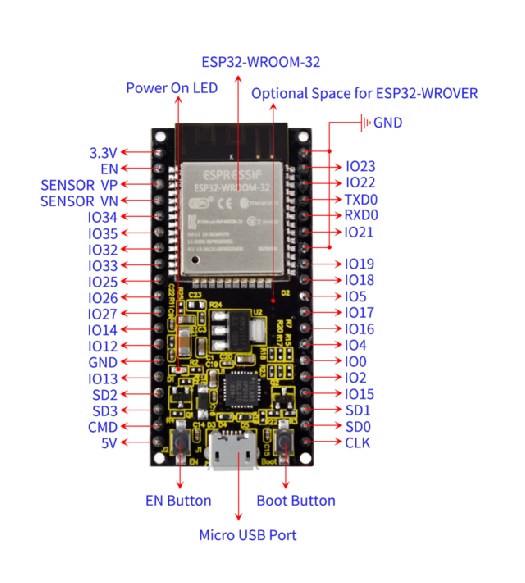
\includegraphics[width=\columnwidth]{./figs/esp32.eps}
\caption{ESP32 Pin Configuration}
\label{fig:arduino}
\end{figure}



\end{document}
